\chapter{Considerações finais}
\label{cap:conclusao}

Redes soma-produto são um modelo relativamente novo e bastante promissor. Ainda há muitas questões teóricas em aberto, como mostrou Peharz em 2015 \cite{Peharz2015}.

Estudar o artigo de Zhao \emph{et al.} \cite{Zhao2015} nos permitiu ter mais compreensão sobre a relação entre redes soma-produto e redes bayesianas. Sabe-se que redes soma-produto e redes bayesianas podem codificar as mesmas distribuições de probabilidade, assim como sabe-se que é bem mais fácil relacionar o tamanho de redes soma-produto com o seu tempo de inferência do que fazer o mesmo com redes bayesianas.

De fato, se definirmos os conceitos de \textbf{compactibilidade} como ``uso de espaço polinomial no número de variáveis'' e \textbf{tratabilidade} como ``tempo de inferência polinomial no número de variáveis'', a partir do resultado de Zhao \emph{et al.} \cite{Zhao2015}, Poupart \cite{Poupart2017} conclui que o conjunto das CPDs representadas por redes soma-produto compactas é igual ao conjunto das CPDs representadas por redes soma-produto tratáveis e do conjunto das CPDs representadas por redes bayesianas tratáveis. Porém, redes bayesianas compactas não necessariamente são tratáveis. Essas relações podem ser vistas na figura \ref{fig:poupart}.

\begin{figure}[h]
  \scalebox{0.8}{
    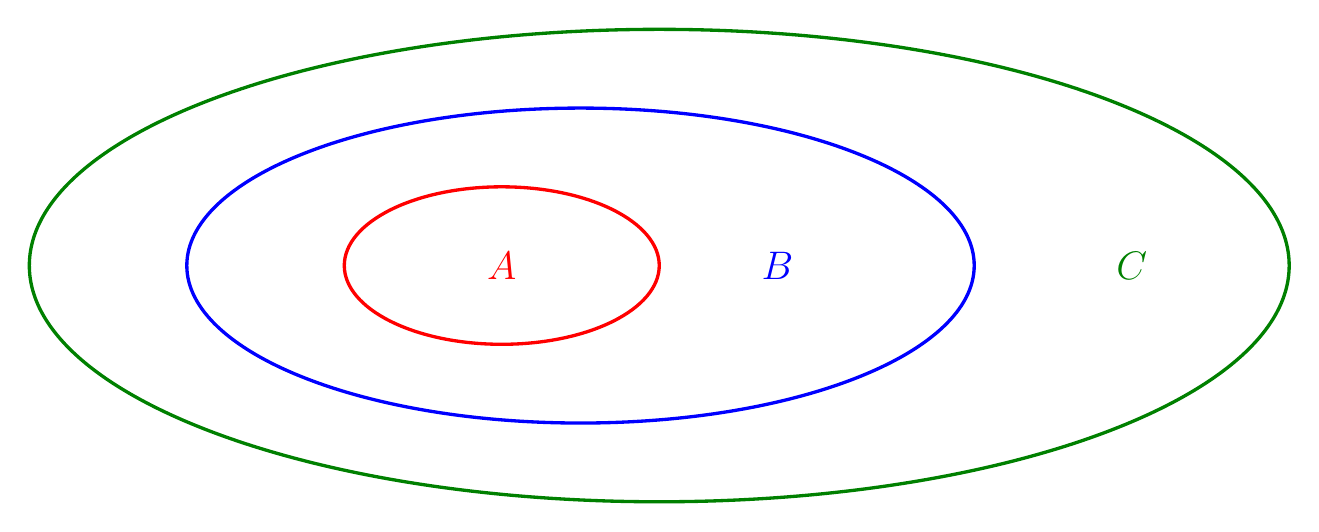
\begin{tikzpicture}
      \draw[very thick,draw=Red] (0,0) ellipse (2cm and 1cm);
      \draw[very thick,draw=Blue] (1cm,0) ellipse (5cm and 2cm);
      \draw[very thick,draw=Green] (2cm,0) ellipse (8cm and 3cm);

      \node[text=Red] at (0,0) {\Large $A$};
      \node[text=Blue] at (3.5cm,0) {\Large $B$};
      \node[text=Green] at (8cm,0) {\Large $C$};
    \end{tikzpicture}
  }

  \vspace{1em}

  \caption{
    \color{Red} $A$: SPNs tratáveis = SPNs compactas = BNs tratáveis.
    \color{Blue} $B$: BNs compactas.
    \color{Green} $C$: SPNs gerais = BNs gerais.
  }

  \label{fig:poupart}
\end{figure}

Embora a implementação do algoritmo de Zhao \emph{et al.} \cite{Zhao2015} --- resultado material deste trabalho --- possa não ter muita aplicação prática neste momento, serviu para facilitar a compreensão do método e para se refletir sobre como representar redes soma-produto e redes bayesianas com diagramas de decisão algébrica utilizando estruturas de dados computacionais.
